\documentclass[12pt]{article}
\renewcommand{\baselinestretch}{1.05}
\usepackage{amsmath,amsthm,verbatim,amssymb,amsfonts,amscd,graphicx,amsrefs}
\usepackage{graphics}
\usepackage{hyperref}
\usepackage{setspace}
\doublespacing
\topmargin0.0cm
\headheight0.0cm
\headsep0.0cm
\oddsidemargin0.0cm
\textheight23.0cm
\textwidth16.5cm
\footskip1.0cm
\theoremstyle{plain}
\newtheorem{theorem}{Theorem}
\newtheorem{corollary}{Corollary}
\newtheorem{lemma}{Lemma}
\newtheorem{proposition}{Proposition}
\newtheorem*{surfacecor}{Corollary 1}
\newtheorem{conjecture}{Conjecture} 
\newtheorem{question}{Question} 
\theoremstyle{definition}
\newtheorem{definition}{Definition}


\begin{document}
\title{Story Time}
\author{by Bart, David, and Gabby}
\maketitle

\section{Introduction}

We wish to find a model of the universe that when hit with rigid motions, continuous or discrete, produces results that agree with the ideas of special relativity. We know (1) the universe is expanding and (2) at some point the universe is expanding at the speed of light. See 
\url{http://w.astro.berkeley.edu/~mwhite/darkmatter/dopplershift.html} \href{http://w.astro.berkeley.edu/}{for more information on the Doppler Shift, the phenomena that leads to these facts.}
We are currently considering two models involving the Klein Disk. 

\subsection{Model One: Disk is Fixed with the Illusion of Expansion}

\begin{figure}[h!]
\centering
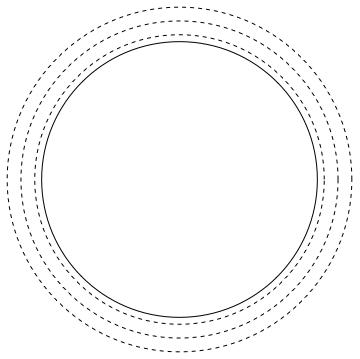
\includegraphics[width=0.3\textwidth]{fixedDisk}
\caption{Klein Disk for Model One}
\end{figure}

\subsection{Model Two: Disk is Expanding}
\begin{figure}[h!]
\centering
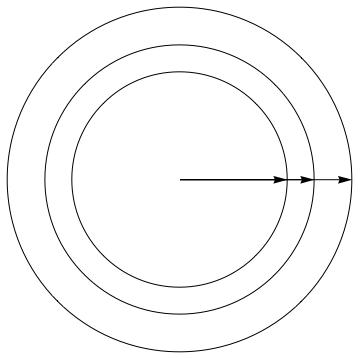
\includegraphics[width=0.3\textwidth]{expandingDisk}
\caption{Klein Disk for Model Two}
\end{figure}

\section{References}
 
\end{document}
 
 
